%%%%%%%%%%%%%%%%%%%%%%%%%%%%%%%%%%%%%%%%%%%%%%%%%%%%%%%%%%%%%%%%%%%%%%%%%%%%%%%%
%2345678901234567890123456789012345678901234567890123456789012345678901234567890
%        1         2         3         4         5         6         7         8

\documentclass[letterpaper, 10 pt, conference]{ieeeconf}  % Comment this line out
                                                          % if you need a4paper
%\documentclass[a4paper, 10pt, conference]{ieeeconf}      % Use this line for a4
                                                          % paper

\IEEEoverridecommandlockouts                              % This command is only
                                                          % needed if you want to
                                                          % use the \thanks command
\overrideIEEEmargins
% See the \addtolength command later in the file to balance the column lengths
% on the last page of the document

\usepackage[utf8]{inputenc} 


 
% The following packages can be found on http:\\www.ctan.org
%\usepackage{graphics} % for pdf, bitmapped graphics files
%\usepackage{epsfig} % for postscript graphics files
%\usepackage{mathptmx} % assumes new font selection scheme installed
%\usepackage{times} % assumes new font selection scheme installed
%\usepackage{amsmath} % assumes amsmath package installed
%\usepackage{amssymb}  % assumes amsmath package installed

\title{\LARGE \bf
VisBig : Visualize Big Data in Real Time
}

%\author{ \parbox{3 in}{\centering Huibert Kwakernaak*
%         \thanks{*Use the $\backslash$thanks command to put information here}\\
%         Faculty of Electrical Engineering, Mathematics and Computer Science\\
%         University of Twente\\
%         7500 AE Enschede, The Netherlands\\
%         {\tt\small h.kwakernaak@autsubmit.com}}
%         \hspace*{ 0.5 in}
%         \parbox{3 in}{ \centering Pradeep Misra**
%         \thanks{**The footnote marks may be inserted manually}\\
%        Department of Electrical Engineering \\
%         Wright State University\\
%         Dayton, OH 45435, USA\\
%         {\tt\small pmisra@cs.wright.edu}}
%}

\author{Gonçalo Fialho \\ 
        Instituto Superior Técnico \\
        Universidade de Lisboa \\ 
        Av. Rovisco Pais, 1049-001 Lisboa, Portugal \\
        Email: goncalo.f.pires@tecnico.ulisboa.pt }
    %    \and  
    %    Gonçalo Fialho \\ 
    %    Instituto Superior Técnico \\
    %    Universidade de Lisboa \\ 
    %    Av. Rovisco Pais, 1049-001 Lisboa, Portugal \\
    %    Email: goncalo.f.pires@tecnico.ulisboa.pt 
    %    }

        % <-this % stops a space
%\thanks{*This work was not supported by any organization}% <-this % stops a space
%\thanks{$^{1}$H. Kwakernaak is with Faculty of Electrical Engineering, Mathematics and Computer Science,
%        Instituto Superior Técnico, Universidade de Lisboa, Portugal
%        {\tt\small h.kwakernaak at papercept.net}}%
%\thanks{$^{2}$P. Misra is with the Department of Electrical Engineering, Wright State University,
%        Dayton, OH 45435, USA
%        {\tt\small p.misra at ieee.org}}%
%}

\makeatletter
\let\NAT@parse\undefined
\makeatother
\usepackage[pdftex]{hyperref}

\usepackage{graphicx}
\begin{document}



\maketitle
\thispagestyle{plain}
\pagestyle{plain}


%%%%%%%%%%%%%%%%%%%%%%%%%%%%%%%%%%%%%%%%%%%%%%%%%%%%%%%%%%%%%%%%%%%%%%%%%%%%%%%%
\begin{abstract}

Nowadays information devices can be found anywhere, whether in a personal computer, smartwatch or even in our appliances. These devices create relevant information to the identification of patterns or anomalies of the systems in question. Given the significant growth of those devices, some display methods are no longer able to respond effectively to users needs. Although there are solutions to visualize this type of information it's important to look for new ways to present them in a real-time environment so users can act quickly to the abrupt change of the regular flow of data so they can attempt to soften or solve the problems of the systems under analysis. This thesis provides a solution for presenting large amounts of real-time data where users are able to identify anomalies and trends in information as well as maintain context when changes in data flow exist.

We propose \textit{VisMillion}, a visualization interface for large amounts of data in real time. Based on \textit{CANVAS} technology that allows graphical rendering through \textit{Javascript}. This web-based approach enables any device that supports HTML5 run the interface without the need of installation of additional libraries, or the existence of OS dependencies. Using different modules the system represents data in many ways. The more recent the data, the more detailed it is, so each module uses different techniques to aggregate and process information. 

This report does a state-of-the-art analysis for viewing large amounts of data in real time. Then it presents the architecture of the solution (backend / real-time and interface / visualization) and its justifications for the options taken. Finally carries out a detailed evaluation of the obtained results and a final analysis and reflection where some of the future work is also mentioned which could improve the system.

Keywords -  Large ammount of data, BigData, Real-Time, Streaming, Visualization, Flow, Trend, Outliers, Patterns

\end{abstract}


%%%%%%%%%%%%%%%%%%%%%%%%%%%%%%%%%%%%%%%%%%%%%%%%%%%%%%%%%%%%%%%%%%%%%%%%%%%%%%%%
\section{INTRODUCTION}


With exponential increase of devices capable of generating information (from the simplest smarthphones to supercomputers) it was necessary to find ways to make the visualization simple and effective, so the user won't be misled by elements that are not part of the data. Many systems create a lot of data that must be analyzed, companies like \textit{Amazon} or \textit{Facebook} need to keep track of all the activities performed by the users so they can interpret trends and patters to create marketing strategies for their business. Robots and Complex Networks generate logs that are important to analyze in case of failures. This is some examples that lead to the emergence of big chunks of information and it is therefore increasingly common to observe the growth of the storage capacity of the devices.

This agglomerated information that creates large chunks of data is typically called as \textbf{Big Data}. However, the term does not have a specific definition and there is no exact value to a dataset can be considered as Big Data \cite{WardB13a}. This data is so large that the tools that process this information cannot do it in a tolerable time interval and its necessary to use more efficient methods. One of the most common uses for this kind of data is to visualize it through representations that show patterns and particular details about them. Its representation can be done from a greater degree of detail of each point to aggregations that describe a lot of points with just an element. Yet, the large amounts of data makes the discovery of relevant items more difficult causing a more complex and time-consuming analysis. Furthermore its hard to represent all the information just in once because the resolution of the displays could not be enough to represent all the points and Humans have difficulties to understand small parts of data when the datasets are huge, losing the context of their search. To overcome this, data is represented with different levels of detail aggregating information at some point. 

The rise of distributed systems raises this problem to a new scale where it is necessary to monitor real-time changes in case of need for rapid intervention in problems that can occur. The more the servers are the more data will exist and each one have different workload making the amount of data generated by second different and that could cause abrupt changes in the visualization of these systems.

There are challenges that visualization of large amounts of data in real time can arise. First, the processing and rendering phases of this data can be slow. Second, unlike a static environment where the data is always on the same spot, real-time data is constantly coming and there is no way to keep the representation state unmodified and explorable like in a fixed dataset. Third, there is no time to wait for new data to process statistics, this process should always be done the fast as possible so the user could retrieve and get the information to act if necessary. Additionally is important to understand the data domain that is visualized so it can be possible to prevent failures and the systems could adapt to data changes so the users cannot be harmed. 

With this in mind we have created VisMillion, which is a interface that represents large amounts of data in real time. Our main goal is to \textbf{provide new information visualization techniques capable of representing large amounts of data in real time that allows the user to perceive the global context of the information as new packages are received}.

The user should be capable to get a global overview of the system and detect interesting patterns using sub visualizations he will explore more details about it. To make this happen the information will be aggregated over time so recent data is always more detailed than the old one, using statistical methods the data is represented in many ways. User should also be capable to identify \textit{outliers} (anomalies) using different methods that are described in the next sections.

The system composed by 3 different modules positioned side by side, each one represents data with a different level of aggregation. Then data flows through each one from right to left. This is built to be suitable with the debit differences and keep updated to all changes that can occur without misleading the user. 

The application was tested using usability user tests with 21 users, using the same approach to all. The results show that the application suits its purpose and the users are capable of analyze changes, patterns and anomalies.

The rest of the paper is organized as follows. Section \ref{section:stateofart} we discuss the related work about real time visualization of large amounts of data. In section \ref{section:streammer} is described the global system architecture and server implementation. In section \ref{section:background} we give a overview about the methods and requirements about information visualization. In section \ref{section:frontend} we present the interface VisMillion. In \ref{section:evaluation} the evaluation of the system is described. Finally, in section \ref{section:conclusions} the conclusions of the work are presented as the future work.




\section{State of the art}
\label{section:stateofart}
Applying real-time to data visualization creates new types of challenges \cite{7994551}. First, we need to understand the data domain, this process is called \textit{Orientation} and we should analyze the data behavior and its components. Second, the systems should react efficiently to data changes that are unexpected, this phase is called \textit{Re-Orientation}.

Information Visualization has three characteristics that should be thought of: \textit{Technique}, \textit{Interactivity}, \textit{Data}. The first one is about \cite{981847} the representation of the data (2D, 3D, pixels, etc.). The interactivity refers how the user should interact with the data to understand the whole system. Data is about its dimensionality and characteristics that influence how data should be presented.

Khan et al. \cite{1878880183} propose a \textit{framework} interact with real-time data capable of dealing with intense data flows. This interface is capable to detect anomalies and highlight them. This approach perform dimensional reduction to the data and then using a recommendation system it chooses the suitable representations for the data. The information uses smooth transitions, so the user can maintain the context about the global data view.

Systems like \cite{traub2017i2, 7338157} use dimensional reduction to deal with large datasets, therefore the interfaces do not have lots of data to render. These processes are commonly performed at server side due to connection issues like latency and protocols. Furthermore, there is some complexities associated with performing dimensional reduction and usually they take some time to process, there are some algorithms to perform this quickly on real-time systems.

Some monitoring systems like LiveRac \cite{McLachlan} and X-SimViz \cite{7338157} create solutions that enables users to visualize and analyze clusters of nodes that need to be supervised in case of something bad happen and Human intervention is required. These applications use multiple views, each one uses different levels of detail or present different types of data. Using techniques like \textit{Brushing \& Linking} and \textit{Stretch and Squish Navigation} each part of the interface can communicate with the others and make the context of the data received being preserved.

\textit{Event Visualizer} \cite{Fischer} is a system capable of processing, analyzing and presenting dynamic events in real-time. It uses a module that pre-processes events and makes a search for missing data. Then the interface categorizes each event and each category corresponds to a bar called \textit{relaxed timeline}. There are multiple \textit{relatex timelines} and each one is binded with a different color, its width corresponds to a time interval. The user uses \textit{Pan \& Zoom} to interact with the system and watch different timelines avoiding big chunks of events.

After all, these systems try to use multiple techniques to deal with real-time and large datasets. Using different interaction techniques the user is able to perform a better exploration, always keeping in mind that the overview of the system should be maintained and using smooth transitions between the views. Data reduction is used to relieve interface workload and make the elements rendering faster. Some of them even use statistical history about past visualization so they can deduce witch idioms are better for some cases. Data analytic users should be capable to understand patterns and anomalies without much effort, so the interfaces need to be simple and consistent while the data is being received and abrupt system changes should never happen. Despite some systems use these techniques to create interfaces, there is some lack of understanding of how to use all this in one because there are a lot of dependencies with each case.



\section{Streamer}
\label{section:streammer}

The system architecture for this project is based on a client-server approach where the client is the interface, and the server (also called streamer) sends the data to the interface. Since the main purpose of this work is related with the representation of the data, it was decided that the system would follow the \textit{fat-client} architecture where the interface is responsible for the data processing. This web implementation allows the system to be run on every machine that has browser support, so there are no OS dependencies and any regular user is capable use the interface.

Using the \textbf{HTML5} it was possible to make a bidirectional connection between the interface and server so they can communicate to each other, the tool used to make this happen is called \textit{WebSockets}. Data is sent by the server, and the interface receives and processes it, for testing purposes the user is capable to communicate with the server to change the data flow, further ahead this implementation can be used to process data from the server with requisites settled by the user.

Figure \ref{fig:server_struct} shows the application architecture, the dataset is retrieved by a python script (\textit{Streamer.py}) that has which later sends each row of the dataset in one packet to the interface via \textit{WebSocket}, the user must identify the address of the streamer, when this connection is established the streamer starts to send the packages. Again, for testing purposes, the data flow can be exchanged by the user, although in a real environment data is received out of order and a flow cannot be defined.

\begin{figure}[h]
    \centering
    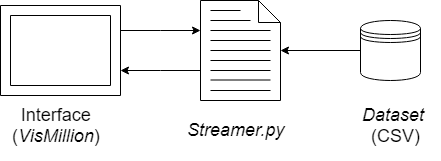
\includegraphics[width=0.9\linewidth]{Figures/server_Structure.png}
    \caption{System architecture}
        \label{fig:server_struct}
\end{figure}

\subsection{Dataset}
\label{subsection:dataset}
Since the purpose of this work is to use a large amount of data to be sent visualized in real-time the dataset to choose must follow two criteria: \textbf{Large} and \textbf{Time-based}. The most common datasets for this are event-based. This data has a timestamp associated (time-based) and one or more attributes, the events can be represented as packages that are sent to the client and then represented. The search of this type of data is facilitated by exponential growth of technology \cite{6567202}, online shopping, social networks and others are always creating this kind of information that can be analyzed and fits perfectly in this case.

It was used two fonts to retrieve this kind of datasets: \textbf{Kaggle} and \textbf{Google BigQuery}. Each one contains multiple time-based data sources with large amounts of data. Using Google BigQuery, it was obtained data related Bitcoin transactions that suit entirely for the system purpose, with this dataset we are able to analyze trends and when there were more transactions occurring or not, as some anomalies that are not in the regular patterns.

The final dataset in CSV format contains hundreds of thousands rows where which one corresponds to transaction value with a timestamp associated. Note this dataset contains only information about half a day of the whole dataset which can be found in Google BigQuery.

\subsection{Usability Tests Server Update}
\label{subsection:usabilityTests}
Due to the need for usability tests to evaluate the system, the server implementation was changed to support data timestamps, so the server could send the data like in a real scenario with different delays between the data dispatch. The retrieved data from the CSV file has now one required field beside the package value, the delta milliseconds between the next package. The server uses this value to set the thread sleep interval between each message sent to the client. This implementation makes more sense than the first one because in the previous approach the interval between each message was always the same, this its very unlikely to happen in a real world context.

\subsection{Dataset Generator}
\label{subsection:datasetGenerator}
The dataset generator is a script create due the need to replicate the exact same tests in usability test phase. So this script generate CSV files with a pair of value and delta .....

% https://www.scribens.com/
% https://www.thesaurus.com/

\section{Background - InfoVis}
\label{section:background}



\section{Front End - Visualization}
\label{section:frontend}

\section{Evaluation}
\label{section:evaluation}

\section{Conclusions}
\label{section:conclusions}



\addtolength{\textheight}{-12cm}   % This command serves to balance the column lengths
                                  % on the last page of the document manually. It shortens
                                  % the textheight of the last page by a suitable amount.
                                  % This command does not take effect until the next page
                                  % so it should come on the page before the last. Make
                                  % sure that you do not shorten the textheight too much.

%%%%%%%%%%%%%%%%%%%%%%%%%%%%%%%%%%%%%%%%%%%%%%%%%%%%%%%%%%%%%%%%%%%%%%%%%%%%%%%%



%%%%%%%%%%%%%%%%%%%%%%%%%%%%%%%%%%%%%%%%%%%%%%%%%%%%%%%%%%%%%%%%%%%%%%%%%%%%%%%%



%%%%%%%%%%%%%%%%%%%%%%%%%%%%%%%%%%%%%%%%%%%%%%%%%%%%%%%%%%%%%%%%%%%%%%%%%%%%%%%%




%%%%%%%%%%%%%%%%%%%%%%%%%%%%%%%%%%%%%%%%%%%%%%%%%%%%%%%%%%%%%%%%%%%%%%%%%%%%%%%%


\bibliographystyle{unsrt}
\bibliography{abstract.bib}

\end{document}
